\chapter{Architecture}
\section{Server}

\begin{figure}[hb]
\centering
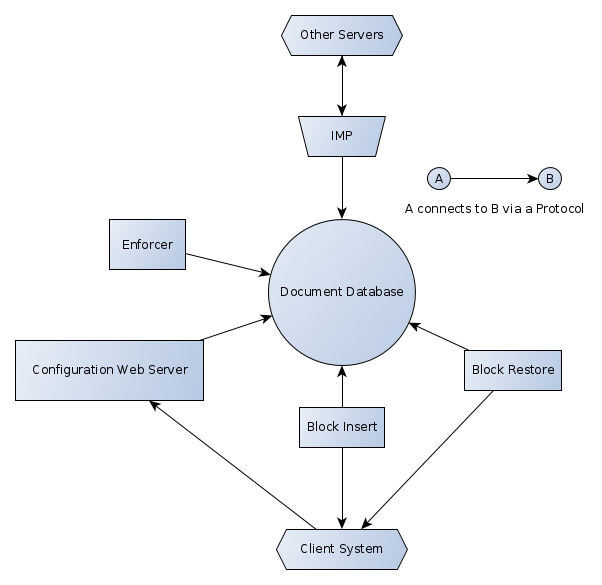
\includegraphics[scale=0.5]{images/architechure-diagram.png}
\caption{A View of the Data Flow Through our Server}
\end{figure}

Our architecture is dual-layer. Each computer connects to a single storage
device and performs all back operations to the device. Each computer will start
an OpenSSH server on boot. This, with the appropriate firewall settings, will
allow the storage device to contact the computer and access its files. The
storage device is made aware of the clients through a packet broadcast by the
client during setup. Once that initiation is complete the backup server can
connect to each client and download each file, block-wise. Each block is stored
in a document-oriented database and stored in a document along with its hash.
Documents associating files with a set of hashes and grouping files with
directories are stored in separate documents. Each computer is represented by a
document that specifies the files in that computer that are backed up in
addition to that computer's scheduling configuration. Once the data and its form
has been successfully stored, the Interface Message Processor is responsible for
finding other storage devices and replicating the data to each device.

\section{Client}
\begin{figure}[hb]
\centering
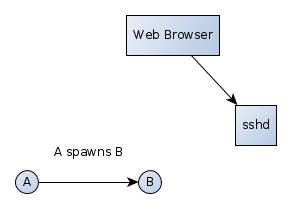
\includegraphics[scale=0.5]{images/client-arcitechure.png}
\caption{A View of Client Architecure}
\end{figure}

The client's job is to find the server and provide a way for the server to connect with the client.

\section{Distribution Algorithm}